\documentclass[10pt, a4paper]{article}
\usepackage{lrec2006}
\usepackage{graphicx}

\usepackage{url}

\usepackage[utf8]{inputenc}
\usepackage{multirow} 
\usepackage[small,bf]{caption} 

%% \usepackage{multibib}
%%\usepackage[comma]{natbib}
%% \usepackage{chapterbib}

\usepackage{lingmacros}
\usepackage{threeparttable}

\usepackage{fancyvrb} 
\DefineVerbatimEnvironment{outputExample}{Verbatim}{fontsize=\small}
\DefineVerbatimEnvironment{goldExample}{BVerbatim}{fontsize=\tiny}

\bibdata{apertium-hbs-slv}

\newcommand{\sentenceexample}[1]{{\small\enumsentence{#1}}}

\title{Shallow-transfer rule-based machine translation for the Western group of South Slavic languages}

\name{Hrvoje Peradin, Filip Petkovsky, Francis M. Tyers}
%\name{X, Y, Z}

%\address{A, B, C}
\address{University of Zagreb, University of Zagreb, Institut for språkvitskap \\
               Faculty of Science, Faculty of Electrical Engineering, Det humanistiske fakultet \\
               Dept. of Mathematics, and Computer Science, N-9037 Universitetet i Tromsø\\
               hperadin@gmail.com, filip.petkovski@fer.hr, ftyers@prompsit.com\\}


\abstract{
The South Slavic languages, spoken mostly in the Balkans, make up one
of the three Slavic branches. The South Slavic branch is in turn
comprised of two subgroups, the Eastern subgroup containing Macedonian
and Bulgarian, and the western subgroup containing Serbo-Croatian
and Slovenian. This paper describes the development of a
bidirectional machine translation system for the western branch of
South-Slavic languages — Serbo-Croatian and Slovenian. Both
languages have a free word order, are highly inflected, and share a
great degree of mutual inteligibility. They are also under-resourced
as regards free/open-source resources. We give details on the resources and
development methods used, as well as an evaluation, and
general directions for future work.
 \\ \newline %\Keywords{keyword A, keyword B, keyword C}
}

\begin{document}

\maketitleabstract


\section{Introduction}

The South Slavic language branch, which is spoken mostly in the
Balkans, makes up one of the three Slavic branches. The South Slavic
branch itself is in turn comprised of two subgroups, the Eastern subgroup
containing Macedonian and Bulgarian, and the western subgroup
containing Serbo-Croatian and Slovenian.

The Serbo-Croatian (\texttt{hbs})\footnote{We use the term `Serbo-Croatian' as an abbreviation for
Bosnian-Croatian-Montenegrin-Serbian.} 
dialects are the native language of most people in Serbia, Croatia, 
Montenegro and Bosnia and Herzegovina. They were formed on the basis of the \emph{štokavian} dialects 
which got their name from the form \emph{što} (or \emph{šta}), which is used for the 
interrogative pronoun `what?'. A second group of dialects from the Serbo-Croatian language group 
is the Čakavian group spoken in western Croatia, Istria, the coast of Dalmatia, and some 
islands in the Adriatic. Like the štokavian dialects, the \emph{čakavian} dialects got their name 
from the form \emph{ča} used for the same interrogative pronoun. Finally, the third main group 
of Serbo-Croatian dialects, spoken in north-western Croatia, uses \emph{kaj} instead of \emph{što}, 
and is called \emph{kajkavian}.
An intermediate dialect between Serbo-Croatian, Bulgarian and Macedonian is the Torlakian dialect.
The three or four standardised varieties of Serbo-Croatian are all based on the štokavian dialect.

Slovenian (\texttt{slv}) is the native language of Slovenia, and is
also spoken in the neighbouring areas in Italy and Austria. While
Slovenian has many different dialects, it shares some features with
the Kajkavian and Čakavian dialects spoken in Croatia. Although the
speakers of the different Serbo-Croatian dialects can understand each
other without any serious difficulties, a Serbo-Croatian speaker can
have a difficult time understanding a speaker of a Slovenian dialect.

\begin{figure}
\centering
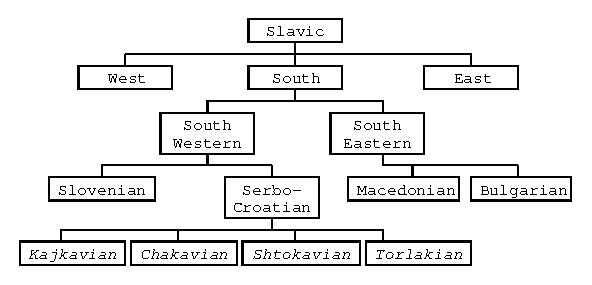
\includegraphics[width=0.5\textwidth]{images/chart.eps}
\caption{A traditional division of the South-Slavic languages. All four standard varieties
     of Serbo-Croatian (Bosnian, Croatian, Montenegrin, and Serbian) are based on the 
     štokavian dialect.}
\end{figure}

\begin{table*}
\centering
\begin{tabular}{lcccc}
  \hline
              &  \textbf{Bosnian} & \textbf{Croatian} & \textbf{Montenegrin} & \textbf{Serbian}\\
  \hline
 \textbf{Čakavian}  & - & -i-,-e-,-je- & - & -  \\
 \textbf{Kajkavian}  & - & -e-,-ie-,-ei,-i- & - & -  \\
 \textbf{Štokavian}  & -ije-,-je- & -ije-,-je-,-i- & -ije-,-je- & -e-,-ije-,-je-  \\
 \textbf{Torlakian}  & - & - & - & -e-  \\
\hline
\end{tabular}
\caption{Intersection of Serbo-Croatian languages and dialects. All four standard variants 
  are based on the štokavian dialect, but other dialects are considered to \emph{belong} to a 
  standard. The -ije-, -e-, and -i- correspond to the \emph{yat} reflex.}
\end{table*}

%% \begin{figure}

%% \todo{Venn diagram of Serbo-Croatian, Serbian, Croatian, Bosnian, Montenegrin, 
%% Neo-Štokavian, Čakavian, Kajkavian, Torlakian
%% Ekavian, Ijekavian, Ikavian}

%% \end{figure}



\section{Design}
\subsection{The Apertium platform}
\nocite{forcada2011apertium}
The Apertium\footnote{\url{http://wiki.apertium.org/}} platform is a
modular machine translation system. The typical core layout consists
of a letter transducer morphological lexicon.\footnote{A list of
ordered pairs of word surface forms and their lemmatised
analyses.} The transducer produces cohorts\footnote{A cohort 
consists of a surface form and one or more readings containing the lemma of the 
word and the morphological analysis.} which are then subjected to a
morphological disambiguation process.
%
Disambiguated readings are then looked up in the bilingual dictionary,
which gives the possible translations for each reading. These
are then passed through a lexical-selection module \cite{tyers12a}, 
which applies rules that select the most appropriate translation
for a given source-language context.
After lexical selection, the readings, which are now pairs of source
and target language lexical forms are passed through a 
syntactic transfer module that performs word reordering, deletions,
insertions, and basic syntactic chunking.
%
The final module is another letter transducer which generates
surface forms in the target language from the bilingual transfer
output cohorts.

\subsection{Constraint Grammar}
This language pair uses a Constraint Grammar (CG)
module\footnote{Implemented in the CG3 formalism, using the
  \texttt{vislcg3} compiler, available under GNU GPL. For a detailed
  reference see: \url{http://beta.visl.sdu.dk/cg3.html}} for
disambiguation. The CG formalism consists of hand-written rules that
are applied to a stream of tokens. Depending on the morphosyntactic
context of a given token the rules select or exclude readings of a
given surface form, or assign additional tags.


% Development; also contains disambiguation, lexical transfer, and structural transfer
\section{Development}

\subsection{Resources}
This language pair was developed with the
aid of on-line resources containing word definitions and flective
paradigms, such as \emph{Hrvatski jezični
  portal}\footnote{\url{http://hjp.srce.hr}} for the Serbo-Croatian side. For
the Slovenian side we used a similar online resource \emph{Slovar
  slovenskega knjižnega
  jezika},\footnote{\url{http://bos.zrc-sazu.si/sskj.html}} and the
\emph{Amebis Besana} flective
lexicon.\footnote{\url{http://besana.amebis.si/pregibanje/}}

The bilingual dictionary for the language pair was developed from scratch,
using the \emph{EUDict}\footnote{\url{http://eudict.com/}} online
dictionary and other online resources.
%\emph{Google Translate}\footnote{\url{http://translate.google.com/}}.

\subsection{Morphological analysis and generation}
The basis for this language pair are the morphological
lexicons for Serbo-Croatian (from
the language pair Serbo-Croatian--Macedonian, {\small{\tt apertium-hbs-mak}}) and Slovenian (from the
language pair Slovenian--Spanish, {\small{\tt apertium-slv-spa}}). Both
lexicons are written in the XML format of
\emph{lttoolbox}\footnote{\url{http://wiki.apertium.org/wiki/Lttoolbox}}
\cite{rojas2005construccion}, and were developed as parts of
their respective language pairs, during the Google Summer of Code
2011.\footnote{\url{http://code.google.com/soc/}} Since the lexicons
had been developed using different frequency lists, and slightly
different tagsets, they have been further trimmed and updated to
synchronise their coverage.

%wiktionaries and Wikipedia, as well as an SETimes corpus\footnote{\url{http://opus.lingfil.uu.se/SETIMES.php}} (\citealp{tyers2010south}) and a%corpus composed from the Serbian, Bosnian, Croatian and Serbo-Croatian Wikipedias.

%% Other resources for morphological analysis of Serbian and Croatian exist
%% (\citealp{vitas2004intex}, \citealp{vitas2003processing}, \citealp{agic2008improving}, \citealp{snajder08automatic}), 
%% to our knowledge there are none freely available for either Serbian, Bosnian or
%% Croatian. 


\subsection{Disambiguation}
Though for both languages there exists a number of tools for
morphological taggin and disambiguation (\todo{reference some}), there
are none freely available. Likewise, the adequatly tagged corpora are
mostly non-free (\todo{reference some non-free corpora, like
  1984.,...}). \todo{See on the taggers/corpora for Slovene}\todo{See
  on the taggers/corpora for BCMS}.  Since both BCMS Slovene are
highly inflected languages, the automatically trained statistical
tagger canonically used in Apertium language pairs would not give
satisfactory results. For this reason we chose to use solely
Constraint Gramar (CG) for disambiguation. The CG module does not
provide complete disambiguation, so in the case of any remaining
ambiguity the system picks the first output analysis.

Due to the similarities between the languages, we were able to
reuse much of the rules developed earlier for BCMS. Following are
some examples of disambiguation rules:

\begin{itemize}
\item Preposition based case disambiguation

\sentenceexample{
Za našo ljubo staro mater. $\leftrightarrow$ Za našu dragu staru majku.

[For{\sc.pr.acc}] [our{\sc.prn.acc}] [dear{\sc.prn.acc}] [old{\sc.prn.acc}] [mother{\sc.n.acc}]

(For our dear old mother.)
}

Noun phrases in both languages typically generate a great number of
ambiguities. For this phrase the morphological analyser gives:

{\small
\begin{Verbatim}
    "<Za>"
         "za" pr acc 
    ;    "za" pr gen
    ;    "za" pr ins
    "<našo>"
         "naš" prn pos p1 f sg acc 
    ;    "naš" prn pos p1 f sg ins
    "<ljubo>"
         "ljub" adj f sg acc ind 
    ;    "ljubo" adv sint
    ;    "ljub" adj nt sg nom ind
    ;    "ljub" adj nt sg acc ind
    ;    "ljub" adj f sg ins ind
    "<staro>"
         "star" adj f sg acc ind 
    ;    "staro" adv sint
    ;    "star" adj f sg ins ind
    ;    "star" adj nt sg nom ind
    ;    "star" adj nt sg acc ind
"<mater>"
         "mati" n f sg acc 
    ;    "mati" n f du gen
    ;    "mati" n f pl gen
\end{Verbatim} 
}


\end{itemize}



\subsection{Lexical transfer}
The lexical transfer was done with an \emph{lttoolbox} letter
transducer composed of bilingual dictionary entries. Additional
paradigms were added to the transducer to compensate for the tagset
notational differences.

\subsection{Lexical selection}

Since there was no adequate and free Slovene -- Serbo-Croatian parallel corpus, 
we chose to do the lexical selection relying only on Apertium's lexical selection module.
For cases not covered by our hand-written rules, the system would choose the lexical 
default from the bilingual dictionary.
We provide examples of such lexical selection rules.

Phonetics based lexical selection: many words from the Croatian and Serbian dialects differ in a single phoneme.
An example are the words \emph{točno} in Croatian and \emph{tačno} in Serbian (engl. \emph{accurate}).
Such differences were solved through the lexical selection module using rules like:

{\small
\begin{Verbatim}
<rule>
    <match lemma="točno" tags="adv.*">
	<select lemma="točno" tags="adv.*"/>
    </match>
</rule>
\end{Verbatim}
}
for Croatian, and
{\small
\begin{Verbatim}
<rule>
    <match lemma="točno" tags="adv.*">
	<select lemma="tačno" tags="adv.*"/>
    </match>
</rule>
\end{Verbatim}
}
for Serbian and Bosnian.

Similarly, the Croatian language has the form \emph{burza} (meaning stock exchange in English), while Serbian and Bosnian have \emph{berza}. 
For those forms the following rules were written:

{\small
\begin{Verbatim}
<rule>
    <match lemma="borza" tags="n.*">
        <select lemma="burza" tags="n.*"/>
    </match>
</rule>
\end{Verbatim}
}
for Croatian, and 
{\small
\begin{Verbatim}
<rule>
    <match lemma="borza" tags="n.*">
	<select lemma="berza" tags="n.*"/>
    </match>
</rule>

\end{Verbatim}
}
for Serbian and Bosnian.

Another example of a phonetical difference are words which have h in Croatian and Bosnian, but v in Serbian.
Such words include \emph{kuha} and \emph{duhan} in Croatian and Bosnian, but \emph{kuva} and \emph{duvan} in Serbian.
Similar rules were written for the forms for \emph{porcelain} (procelan in Serbian and porculan in Croatian), 
\emph{salt} (so and sol) etc.

While the Serbian dialect accepts the Ekavian and Ikavian reflexes, 
the Croatian dialect uses only the Ijekavian reflex.
Since the selection for the different reflexes of the yat vowel is done in the generation process,
no rules were needed in the lexical selection module.

Internationalisms have been introduced to Croatian and Bosnian mainly through the Italian and German language
whereas they have entered Serbian through French and Russian. 
As a result, the three dialects have developed different phonetic patterns for internatonal words.

Examples of rules for covering such varieties include:
{\small
\begin{Verbatim}
<rule>
    <match lemma="Betlehem" tags="np.*">
	<select lemma="Betlehem" tags="np.*"/>
    </match>
</rule>
\end{Verbatim}
}
for Croatian and Bosnian, and
{\small
\begin{Verbatim}
<rule>
    <match lemma="Betlehem" tags="np.*">
	<select lemma="Vitlejem" tags="np.*"/>
    </match>
</rule>
\end{Verbatim}
}
for Serbian.

Finally, the Croatian months used for the Gregorian calendar have Slavic-derived names and differ from the original Latin names.
For example, the Croatian language has the word \emph{siječanj} for \emph{January}, and 
the Serbian language has the word \emph{Januar}.
These differences were also covered by the lexical selection module.

Besides the yat reflex, several other cases were not covered in the lexical selection module. These include the pronoun "what" which has the form "što" in Croatian and the forms "što" and "šta" in Serbian and Bosnian, depending on whether the context is interrogative or relative. This ambiguity was left out of the lexical selection module and was dealth with during generation.

In Croatian with modal verbs the infinitive is prescribed while in Serbian the construct da + present is usually used.
For example the Croatian translation of the sentence "I want to eat" is "Želim \emph{jesti}", while the Serbian translation is "Želim \emph{da jedem}". This difference was not covered in the lexical selection module.






\subsection{Transfer}

The BCMS and Slovene languages are very closely related, and their
morphologies are extremely similar. Most of non-technical transfer
rules are thus written only for rare syntactic differences. These are
mostly about clitic ordering, and different noun case usage.

Following are examples of transfer rules, which also illustrate some
contrastive characteristics of the languages:

\begin{itemize}
\item The future tense:
\enumsentence{

Ja ću gledati\footnote{The encliticised future tense forms (gledat ću / gledaću) are handled equally.} $\rightarrow$ Jas bom gledal

[I] [will{\sc.clt.p1.sg}] [watch{\sc.inf}] $\rightarrow$ [I] [will{\sc.clt}] [watch{\sc.pres.p1.sg}]

(I will watch.)
}
\end{itemize}


% Tables:

\begin{table}

\begin{center}
\begin{tabular}{|l|rrr|}
\hline
\textbf{Dictionary} & \textbf{Paradigms} & \textbf{Entries} & \textbf{Forms} \\
\hline
Serbo-Croatian &  1,033 & 13,206 & 233,878 \\
Slovenian &  1,909 & 13,383 & 147,580 \\
\hline
Bilingual &  69 &  16,434 & -- \\
\hline
\end{tabular}
\caption{Statistics on number of lexicon entries for each of the dictionaries in the 
   system.}
\label{table:lexicons}
\end{center}

\end{table}

\begin{table}
\begin{center}
\begin{tabular}{|l|rr|}
\hline
 \textbf{Type}      & \texttt{hbs}$\rightarrow$\texttt{slv} & \texttt{slv}$\rightarrow$\texttt{hbs}\\
\hline
Disambiguation      &     194              &     28 \\
Lexical selection   &     --            &  42 \\
Transfer            &                47 &  98 \\
\hline

\end{tabular}
 \caption{Statistics on the number of rules in each direction. For the lexical selection rules, 
   the number indicates that there are 42 rules for each of the three standard varieties currently
   supported.}
\label{table:rules}
\end{center}
\end{table}

% EVALUATION 
\section{Evaluation}
% Hrvatski -> Slovenski
\begin{table}
\begin{tabular}{lrr}

\textbf{Language} & \textbf{SETimes} & \textbf{Europarl}\\
\hline
Serbo-Croatian & 85.41\% & -- \\
Slovenian &  -- & 95.50\%\\
\hline
\end{tabular}
\caption{ Naïve coverage }
\label{table:coverage}
\end{table}


This sections covers the evaluation of the developed system. 
The system was tested by measuring the lexical coverage, and by performing
a qualitative and a quantitative evaluation. 

Lexical coverage tested using existing free corpora, 
while the quantitative evaluation was performed on 100 postedited sentences from the Slovenian news portal 
Delo \footnote{\url{http://www.delo.si/}}.


\subsection{Lexical coverage}

Coverage for the Serbo-Croatian--Slovenian language pair was measured using both the SETimes \citep{tyers2010south} and Europarl \citep{koehn05a} corpora. 
We measured coverage naively, meaning that we assume a word is in our 
dictionaries if at least one of its surface forms is found in the corpus. 
We are aware of the shortcomings of such an evaluation framework, 
however we decided to use it because of its simplicity.

The Serbo-Croatian $\rightarrow$ Slovenian side was evaluated using the SETimes and Europarl corpora. On the other hand,
as SETimes does not cover Slovenian
the Slovenian $\rightarrow$ Serbo-Croatian side was evaluated only on the EuroParl corpus. The results are shown in table \ref{table:coverage}.

\subsection{Quantitative}

The quantitative evaluation was performed by 5 articles
from the slovenian news portal Delo.
The articles were translated from slovenian using Apertium, and were later corrected by a human post-editor in order to get a correct translationn.
Both the word error rate (WER) and position-independent error rate (PER) were calculated
by counting the number of insertions, substitutions and deletions between the post-edited articles
and the original translation. We used the freely available apertium-eval-translator for calculating the WER and PER.
We also reported the percentage of out of vocabulary words (OOV), and the total number of words per article.
The results are given in tables \ref{table:quantitative1} and \ref{table:quantitative2}

We also calculated both metrics for the output of Google Translate\footnote{\url{http://translate.google.com/}} 
and the results are presented in the same tables. 

Given all the assumptions the WER and PER matrics make, the results show that our system is comparable to Google Translate
with regards to translation quality. The Slovenian $\rightarrow$ Serbo-Croatian translation seems to be better than the Serbo-Croatian $\rightarrow$ Slovenian one
which is due to the fact that more effort was put into developing the former direction.


% cp /path/to//apertium//trunk/apertium-eval-translator/WER.pl /path/to/bin
% perl apertium//trunk/apertium-eval-translator/bootstrap_resampling.pl -n 1000 -e /path/to//apertium//trunk/apertium-eval-translator/wer.sh -s SOURCE_FILE -t TEST_FILE -r REF_FILE

\begin{table*}
\begin{center}
\begin{tabular}{|l|r|rr||rr|}
   \hline
  \multirow{2}{*}{\textbf{Article}}  & \multirow{2}{*}{\textbf{Words}} & \multicolumn{2}{|c||}{\textbf{\%~OOV}} & \multicolumn{2}{c|}{\textbf{WER}}\\\cline{3-6}
                    &                & Apertium & Google &  Apertium & Google \\
   \hline
   \hline
  \texttt{maraton}  & 243            & 16.8     & --     & \textbf{[42.85, 47.92]} & [64.39, 74.56] \\
  \texttt{sonce}    & 169            & 17.7     & --     & \textbf{[32.65, 45.33]}    & [47.27, 58.62] \\
  \texttt{merkator} & 414            & 16.9     & --     & \textbf{[38.78, 48.14]}     & [56.13, 70.30] \\
  \texttt{volitve}  & 229            & 13.9     & --     & [37.81, 53.36]      & [46.66, 62.67] \\
%  \texttt{jame}     & 994            & 14.9     & --     & ??      & [57.28, 67.65] \\
                                                           % 49.57	
  \hline
  \hline
  \texttt{maraton}  & 245            & 37.7     & --     & [52.78, 56.25]           & [45.58, 63.87]\\
  \texttt{sonce}    & 171            & 17.5     & --     & [47.50, 62.79]    & [32.10, 58.49] \\
  \texttt{merkator} & 424            & 12.9     & --     & [45.78, 56.56]    & [48.46, 64.15] \\
  \texttt{volitve}  & 226            & 16.8     & --     & [47.00, 58.44]    & [38.09, 58.10]\\
%  \texttt{jame}     & 1,005          & 15.9     & --     & [??, ??]              & [??,??]\\

  \hline
\end{tabular}
 \caption{Results for Word Error Rate (WER) in the Slovenian$\rightarrow$Serbo-Croatian direction (top) and Serbo-Croatian$\rightarrow$Slovenian (bottom). Scores in bold show a statistically significant improvement over the other system according to bootstrap resampling at $p = 0.95$.}
\label{table:quantitative1}
\end{center}
\end{table*}




\subsection{Qualitative}
The biggest problems are currently caused by the incompleteness of our dictionaries.
The issues caused by OOV words are twofold.
The less important issue is the fact that the system is unable to provide a translation for the unknown words. 
However, the more important issue is that OOV words cause problems with disambiguation and transfer, since they
break long chains of words into smaller ones and drastically reduce context information. 

Next, we have seen that the number of disambiguation rules for Slovenian is not sufficient for high quality disambiguation. 
The constraint grammar for the Slovenian side was written based on the constraint grammar for the Serbo-Croatian side,
and it needs further work.

We have also noticed difficulties in the transfer because of the loose grammar of both sides.
Adding additional rules does not significantly improve the performance of the system 
and OOV words make long transfer rules irrelevant.

Finally, beacause of the small timeframe, we were not able to work much on lexical selection.
Our lexical selection module is the least developed part of our system. 
We have not done any work on the Slovenian side and the number of rules for the Serbo-Croatian side is small.
This is due to the fact that no reliable parallel corpus exists for this language pair.






% CONCLUSIONS AND FUTURE WORK
\section{Future work}

The greatest difficulties for our system are caused by the long phrases present 
and the loose and free word order in the South Slavic languages.
Because of that, in future we plan to put more effort into dealing with those problems.
We are aware of the fact that it is difficult to write transfer rules between the two sides,
and we intend to address that issue by first improving the coverage of our dictionaries.

After expanding the dictionaries, we intend to put more time into developing the Slovenian constraint grammar,
and improve transfer by taking into account wider context.

We intend to work on more Slavic language pairs, including Serbo-Croatian--Russian,
and improve our existing ones, including Serbo-Croatian--Macedonian \citep{peradin12} using the 
resources and knowledge obtained by developing this language pair.

Finally, we will keep the resources updated based on the latest politico-linguistic developments,
and we will add the Montenegrin language once the standard is completely agreed on.


%mention different word order, long phrases, difficult to write rules for
%improve coverage, disambiguation (esp. for slv) and transfer rules
%work on more Slavic language pairs (e.g. hbs-rus)
%backport improvements in the HBS components to hbs-mak
%keep up-to-date with latest politico-linguistic developments. Add in
% Montenegrin when the standard is agreed on.
%small timeframe, disambiguation and transfer rudimentary

\section{Conclusions}

This language pair was an encouraging take on a pair of closely
related South-Slavic languages, and represents a satisfying conclusion
to an MT chain of neighbouring languages (the pairs Serbo-Croatian--Macedonian 
and Macedonian--Bulgarian are also available in Apertium). While we are aware that it
is still in its infancy, and has many flaws, it is a valuable
free/open-source resource, and will serve as another solid ground for NLP
in this language group.



\section*{Acknowledgements}

The development of this language pair was funded as a part of the
Google Summer of Code.\footnote{\url{http://code.google.com/soc/}}
Many thanks to the language pair co-author Ale\v{s} Horvat and his
mentor Jernej Vičič, and other Apertium contributors for their
invaluable help and support.


%\nocite{*}

\bibliographystyle{lrec2006}
\bibliography{apertium-hbs-slv}

\end{document}

